\section{Empirical evaluation}
\label{sec:results}
We demonstrate the ability of Composable Energy Surrogates (CES) to efficiently produce accurate solutions. We consider the systems constructed in \citet{overvelde2014relating}: structures with an $8\times8$ array of pores, corresponding to a $4\times4$ assembly of our surrogates, each representing a $2\times2$-pore component. We sample pore shapes from a uniform distribution over valid shapes defined in \citet{overvelde2014relating}. For \textsc{DAgger}, we sample vertical axial strain magnitudes from $\mathcal{U}(0., 0.3)$, and apply compression with probability $0.8$ (as compressive displacements involve more interesting pore collapse) or tension with probability $0.2$.

We compare our composed surrogates to finite element analysis with different-fidelity meshes under axial compression and tension with a macroscopic displacement of~$0.125 L_0$, where~$L_0$ is the original length of the solid. See the appendix for details of the finite element meshes. We use seven pore shapes: $\xi=(0, 0)$, corresponding to circular pores, and six $\xi$ sampled from a uniform distribution over pore parameters defined as valid in \citet{overvelde2014relating}.
\begin{figure*}[h]
 \begin{tabular}{cc}
	 {\resizebox{0.45\textwidth}{!}{
 \begin{adjustbox}{clip, trim=.4cm .3cm .7cm .3cm}
	 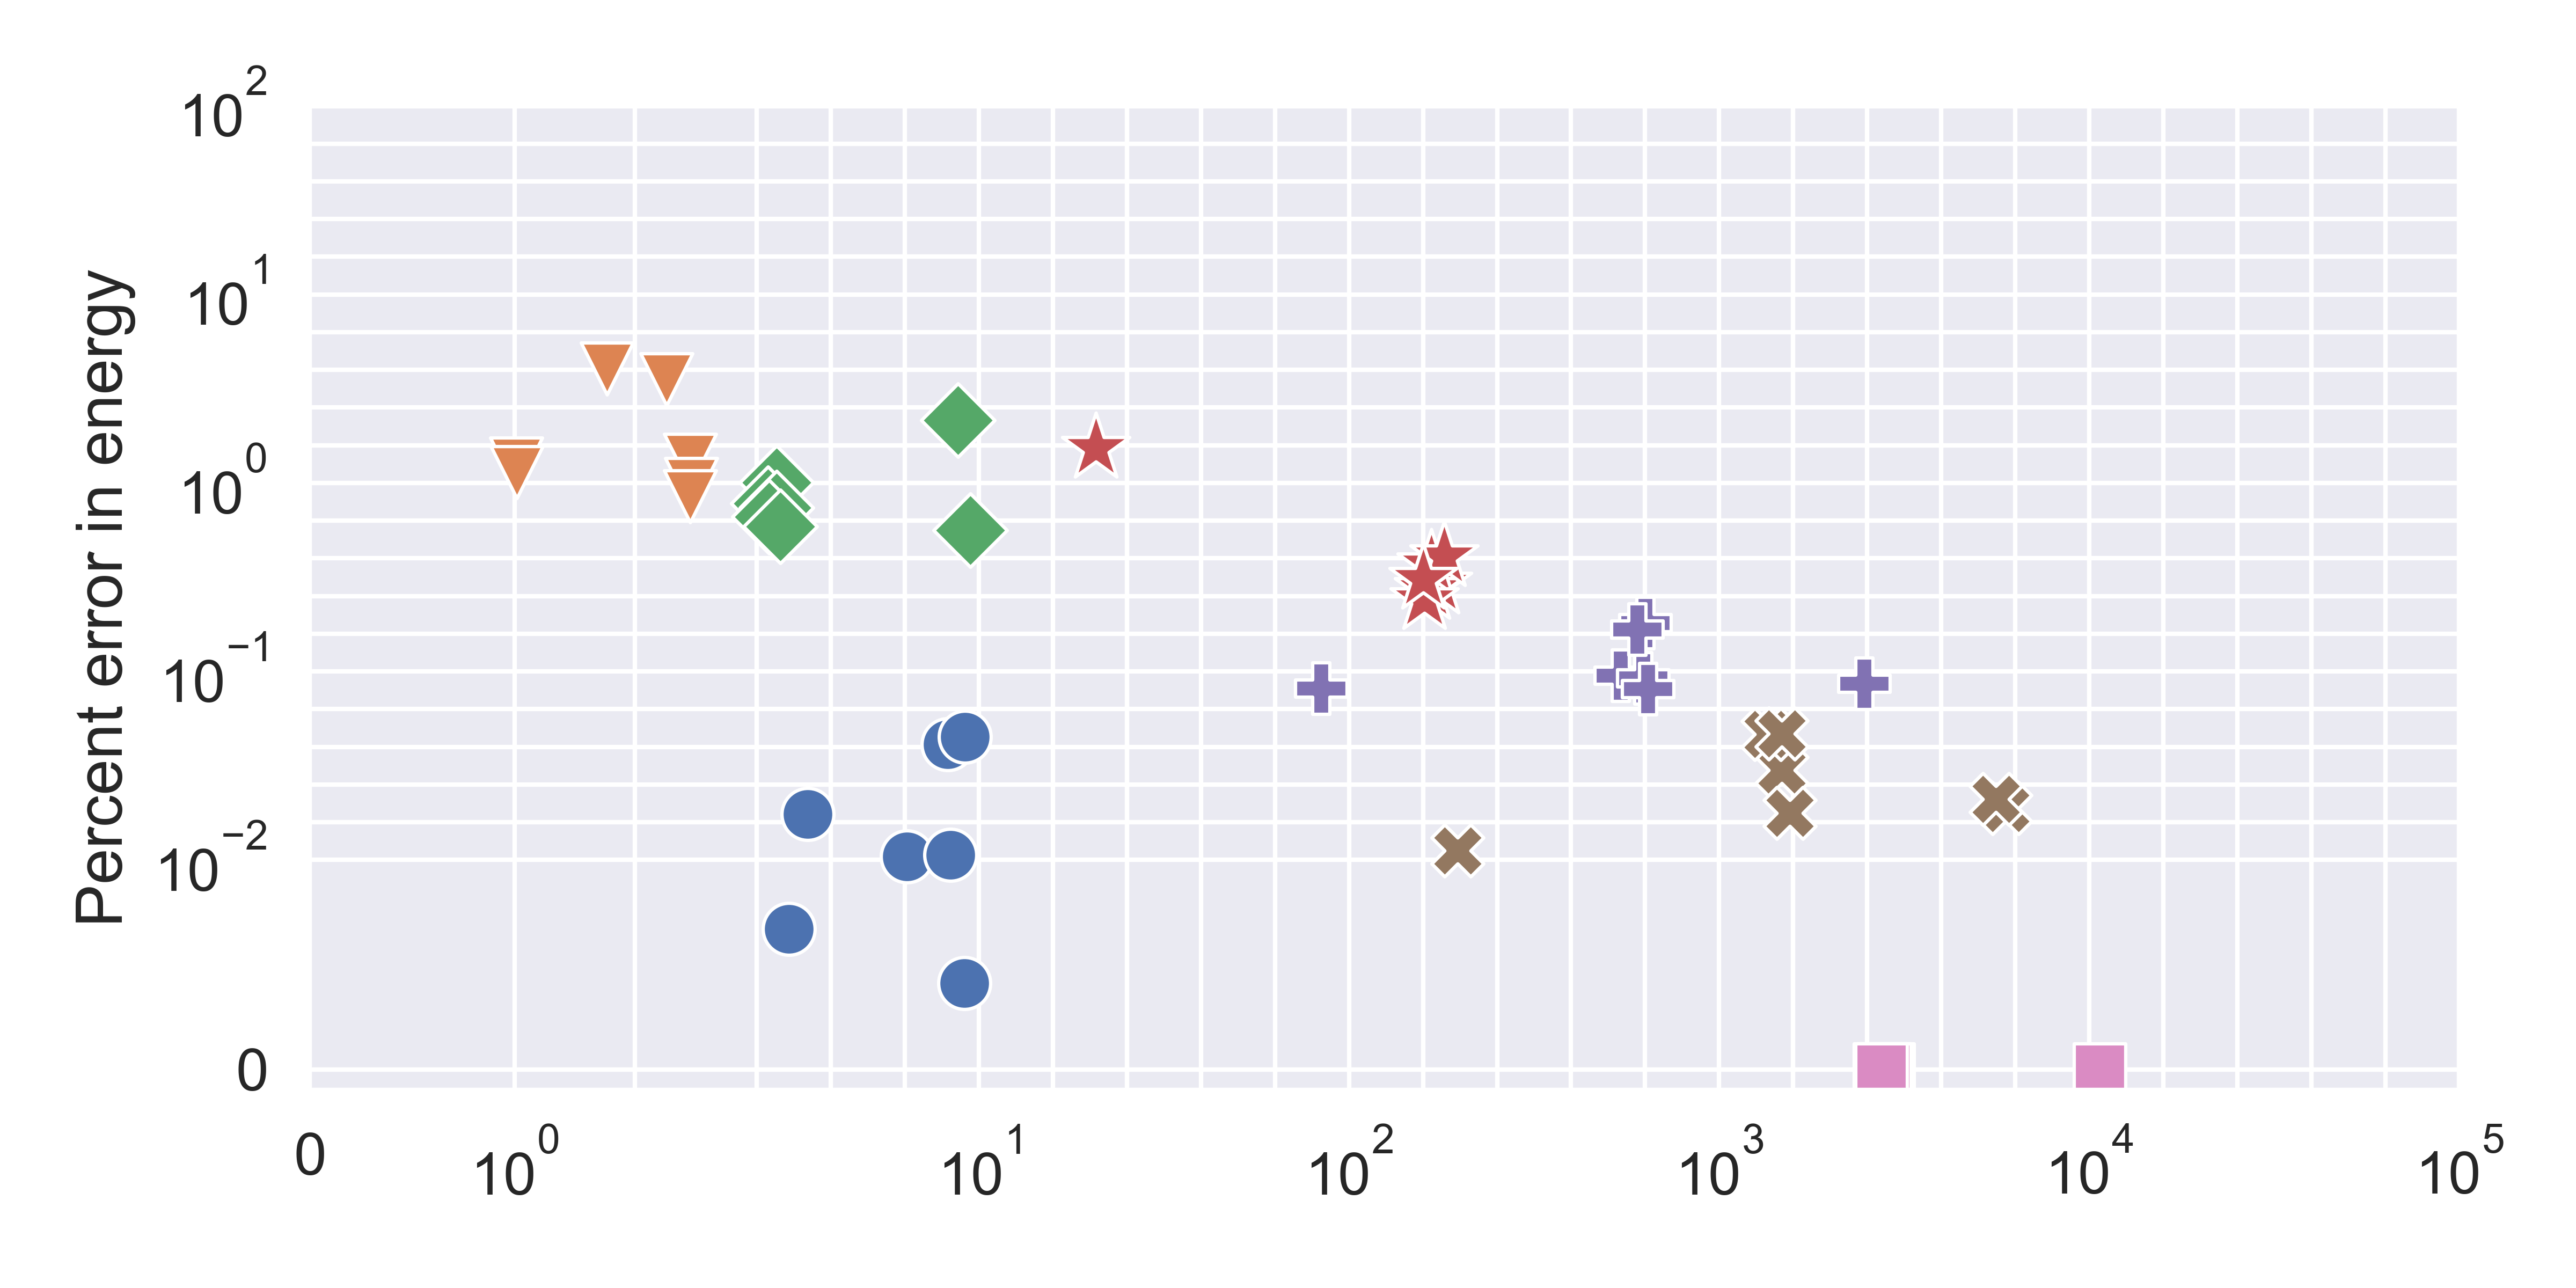
\includegraphics{lces/figures/compression_E.png}
	 \end{adjustbox}
	 }}&
	{\resizebox{0.45\textwidth}{!}{
 \begin{adjustbox}{clip, trim=.4cm .3cm .7cm .3cm}
	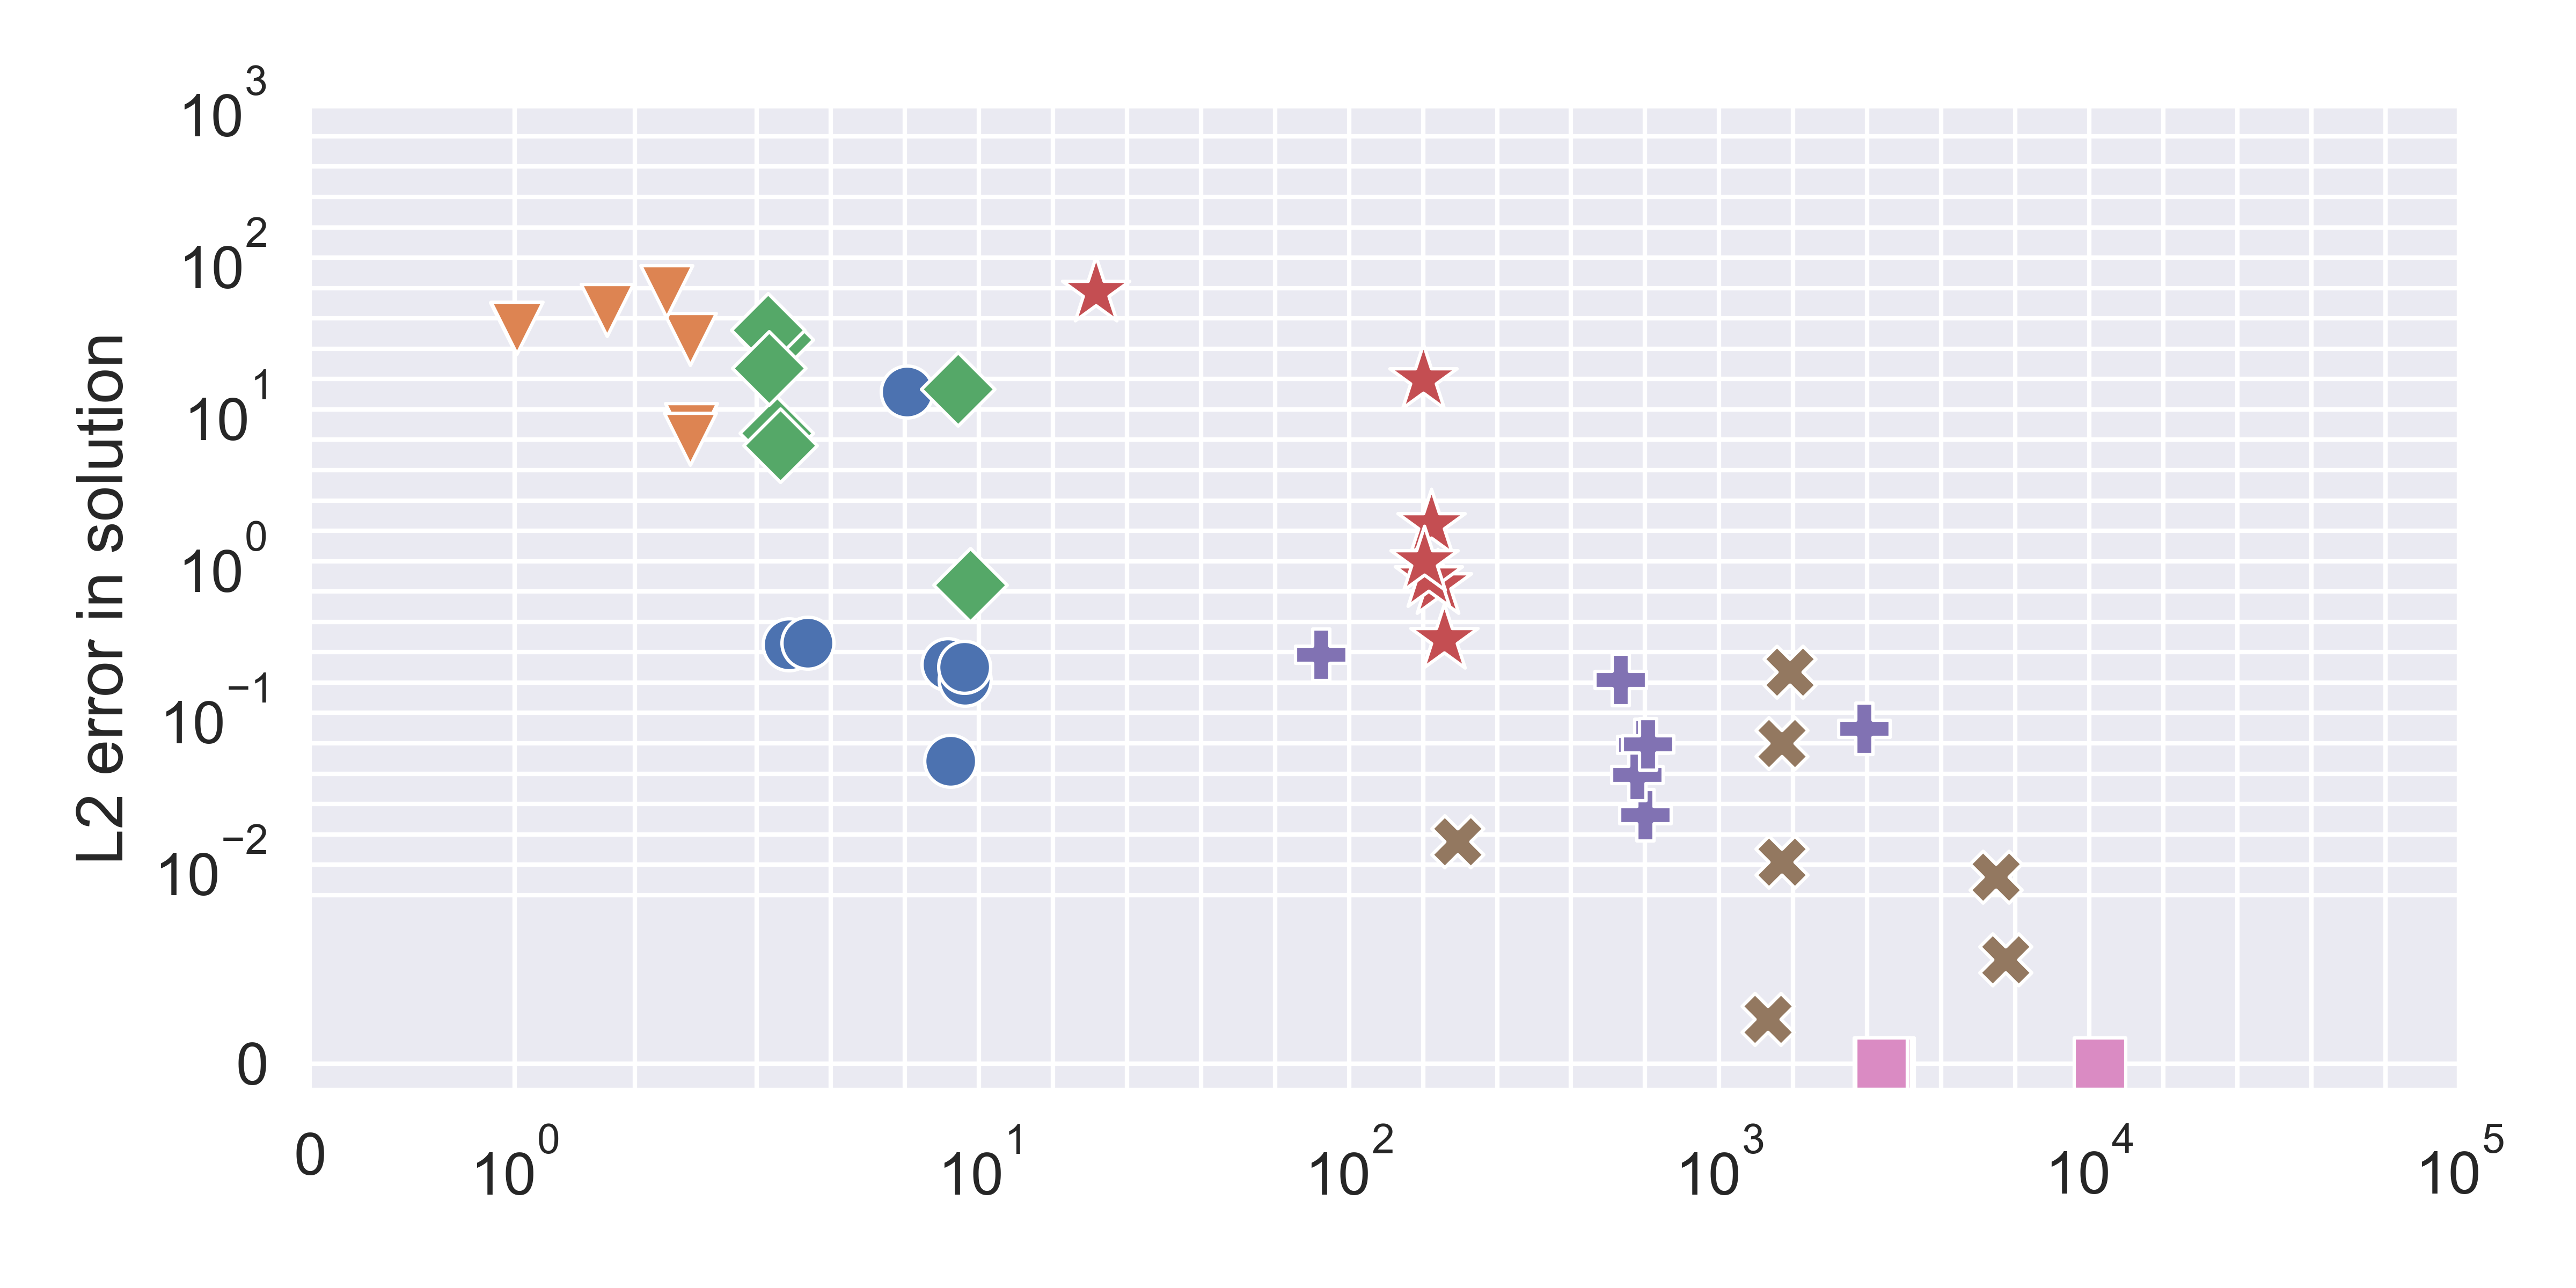
\includegraphics{lces/figures/compression_err.png}
	 \end{adjustbox}
	}}\\
%\rule{0pt}{13ex}
{\resizebox{0.45\textwidth}{!}{
 \begin{adjustbox}{clip, trim=.3cm 0cm .7cm .3cm}
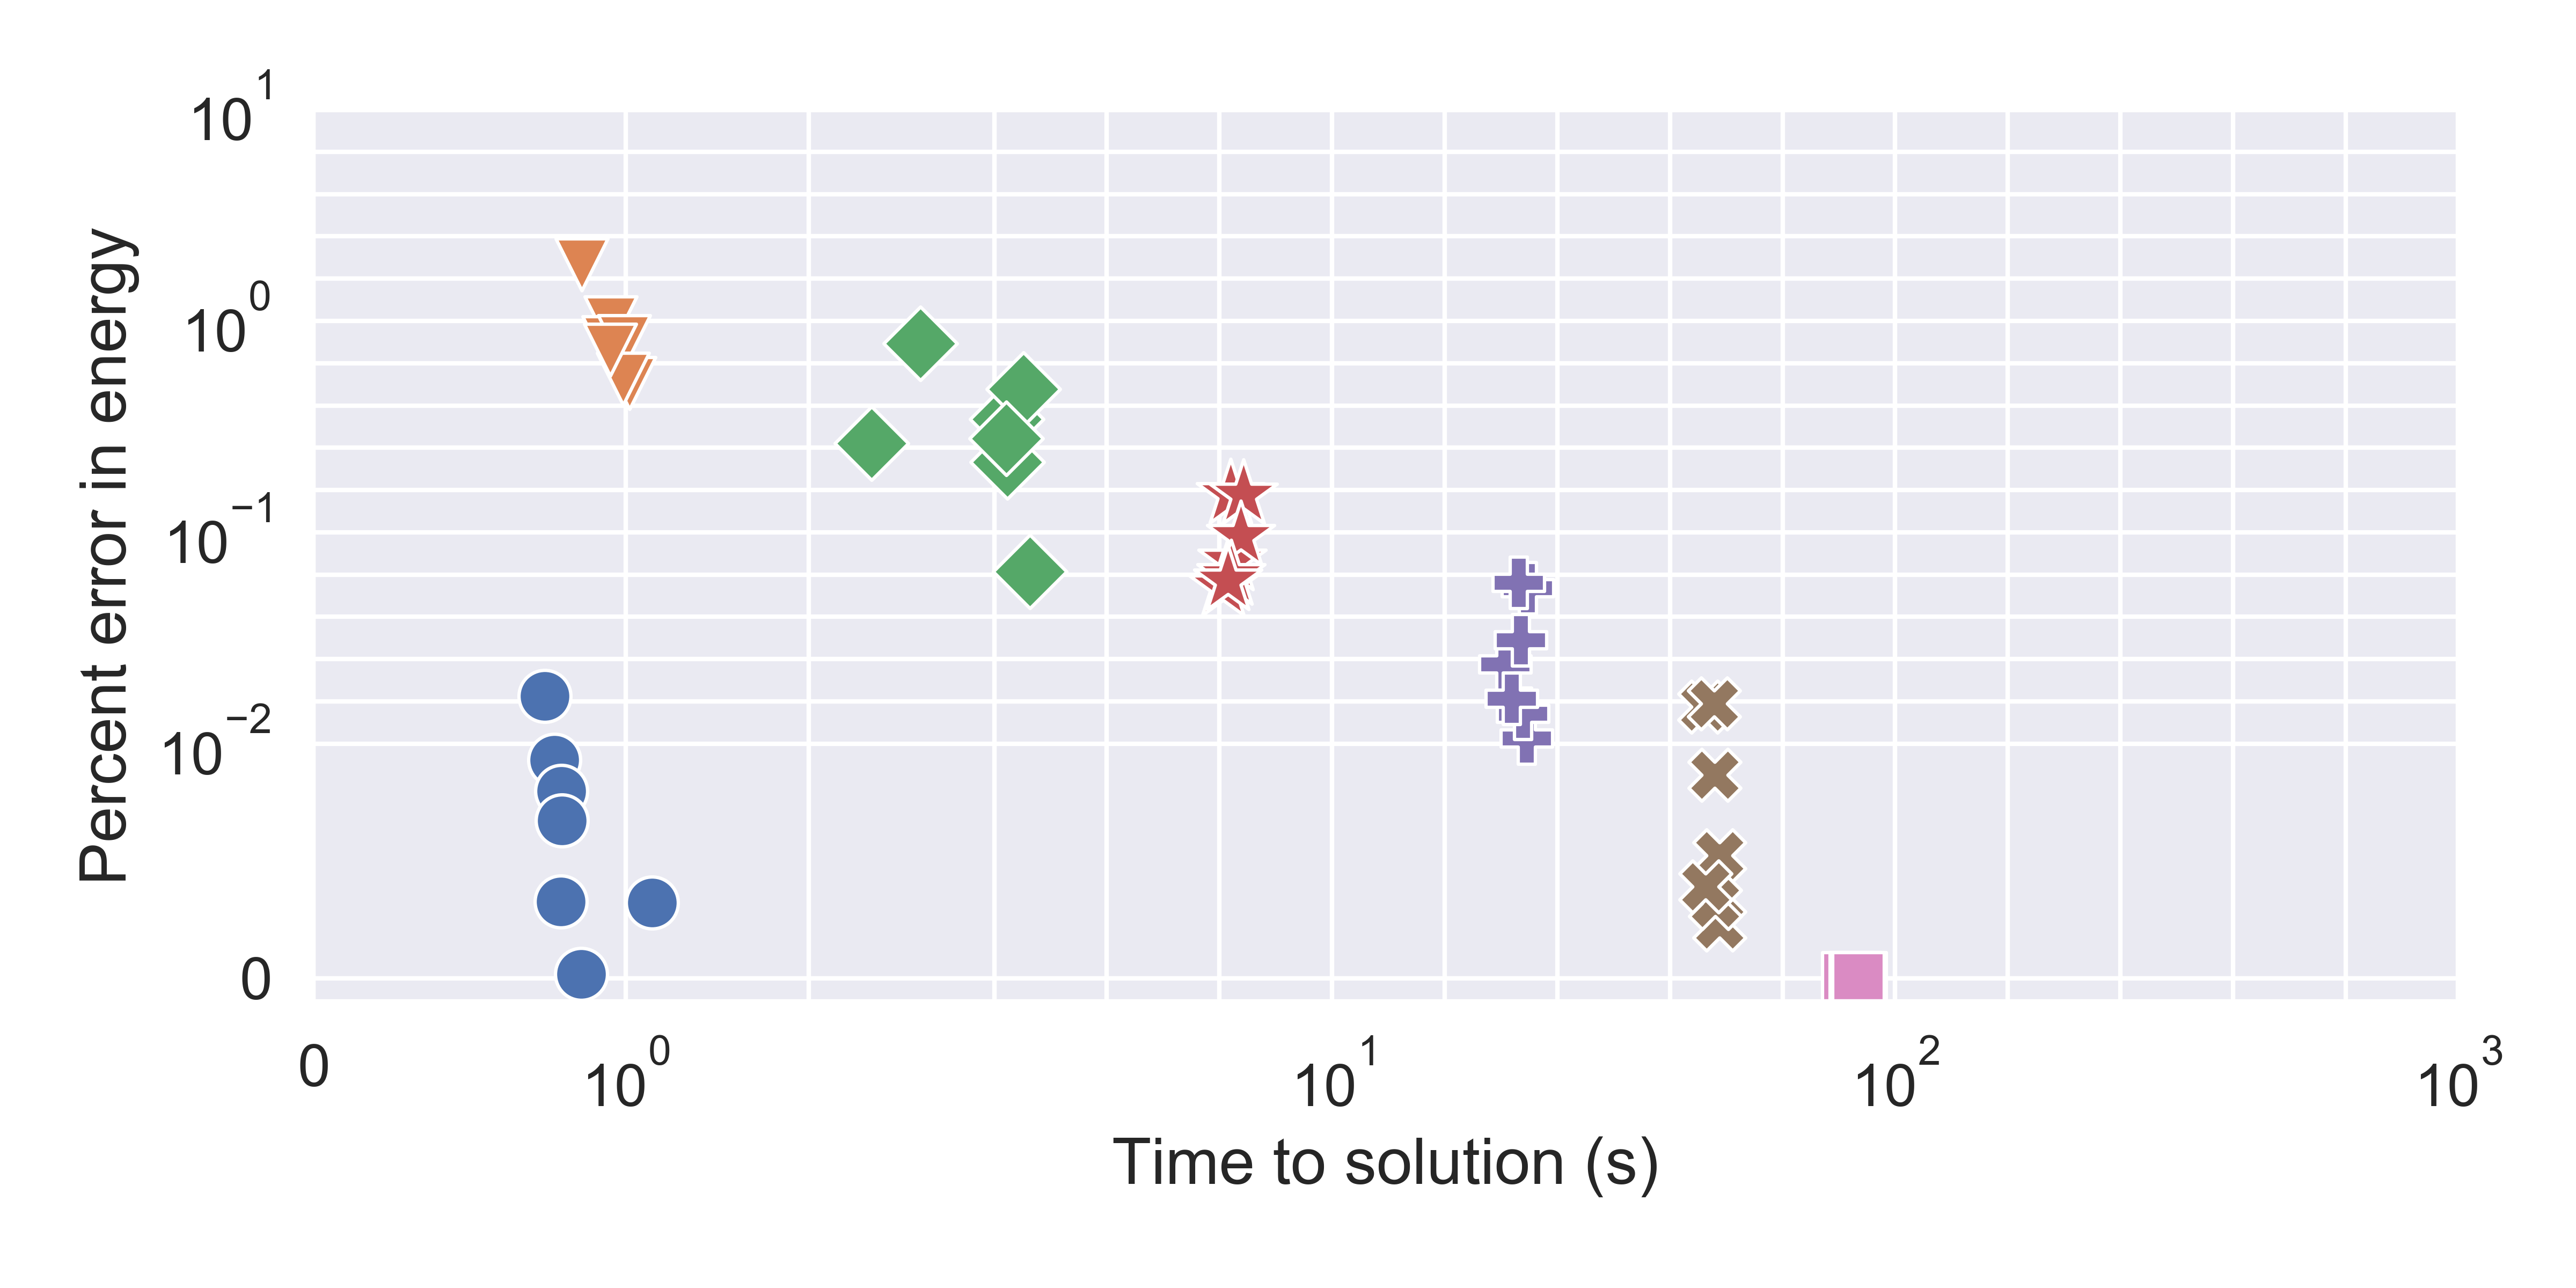
\includegraphics{lces/figures/tension_E.png}
 \end{adjustbox}
}}&%
	{\resizebox{0.45\textwidth}{!}{
 \begin{adjustbox}{clip, trim=.3cm 0cm .7cm .3cm}
	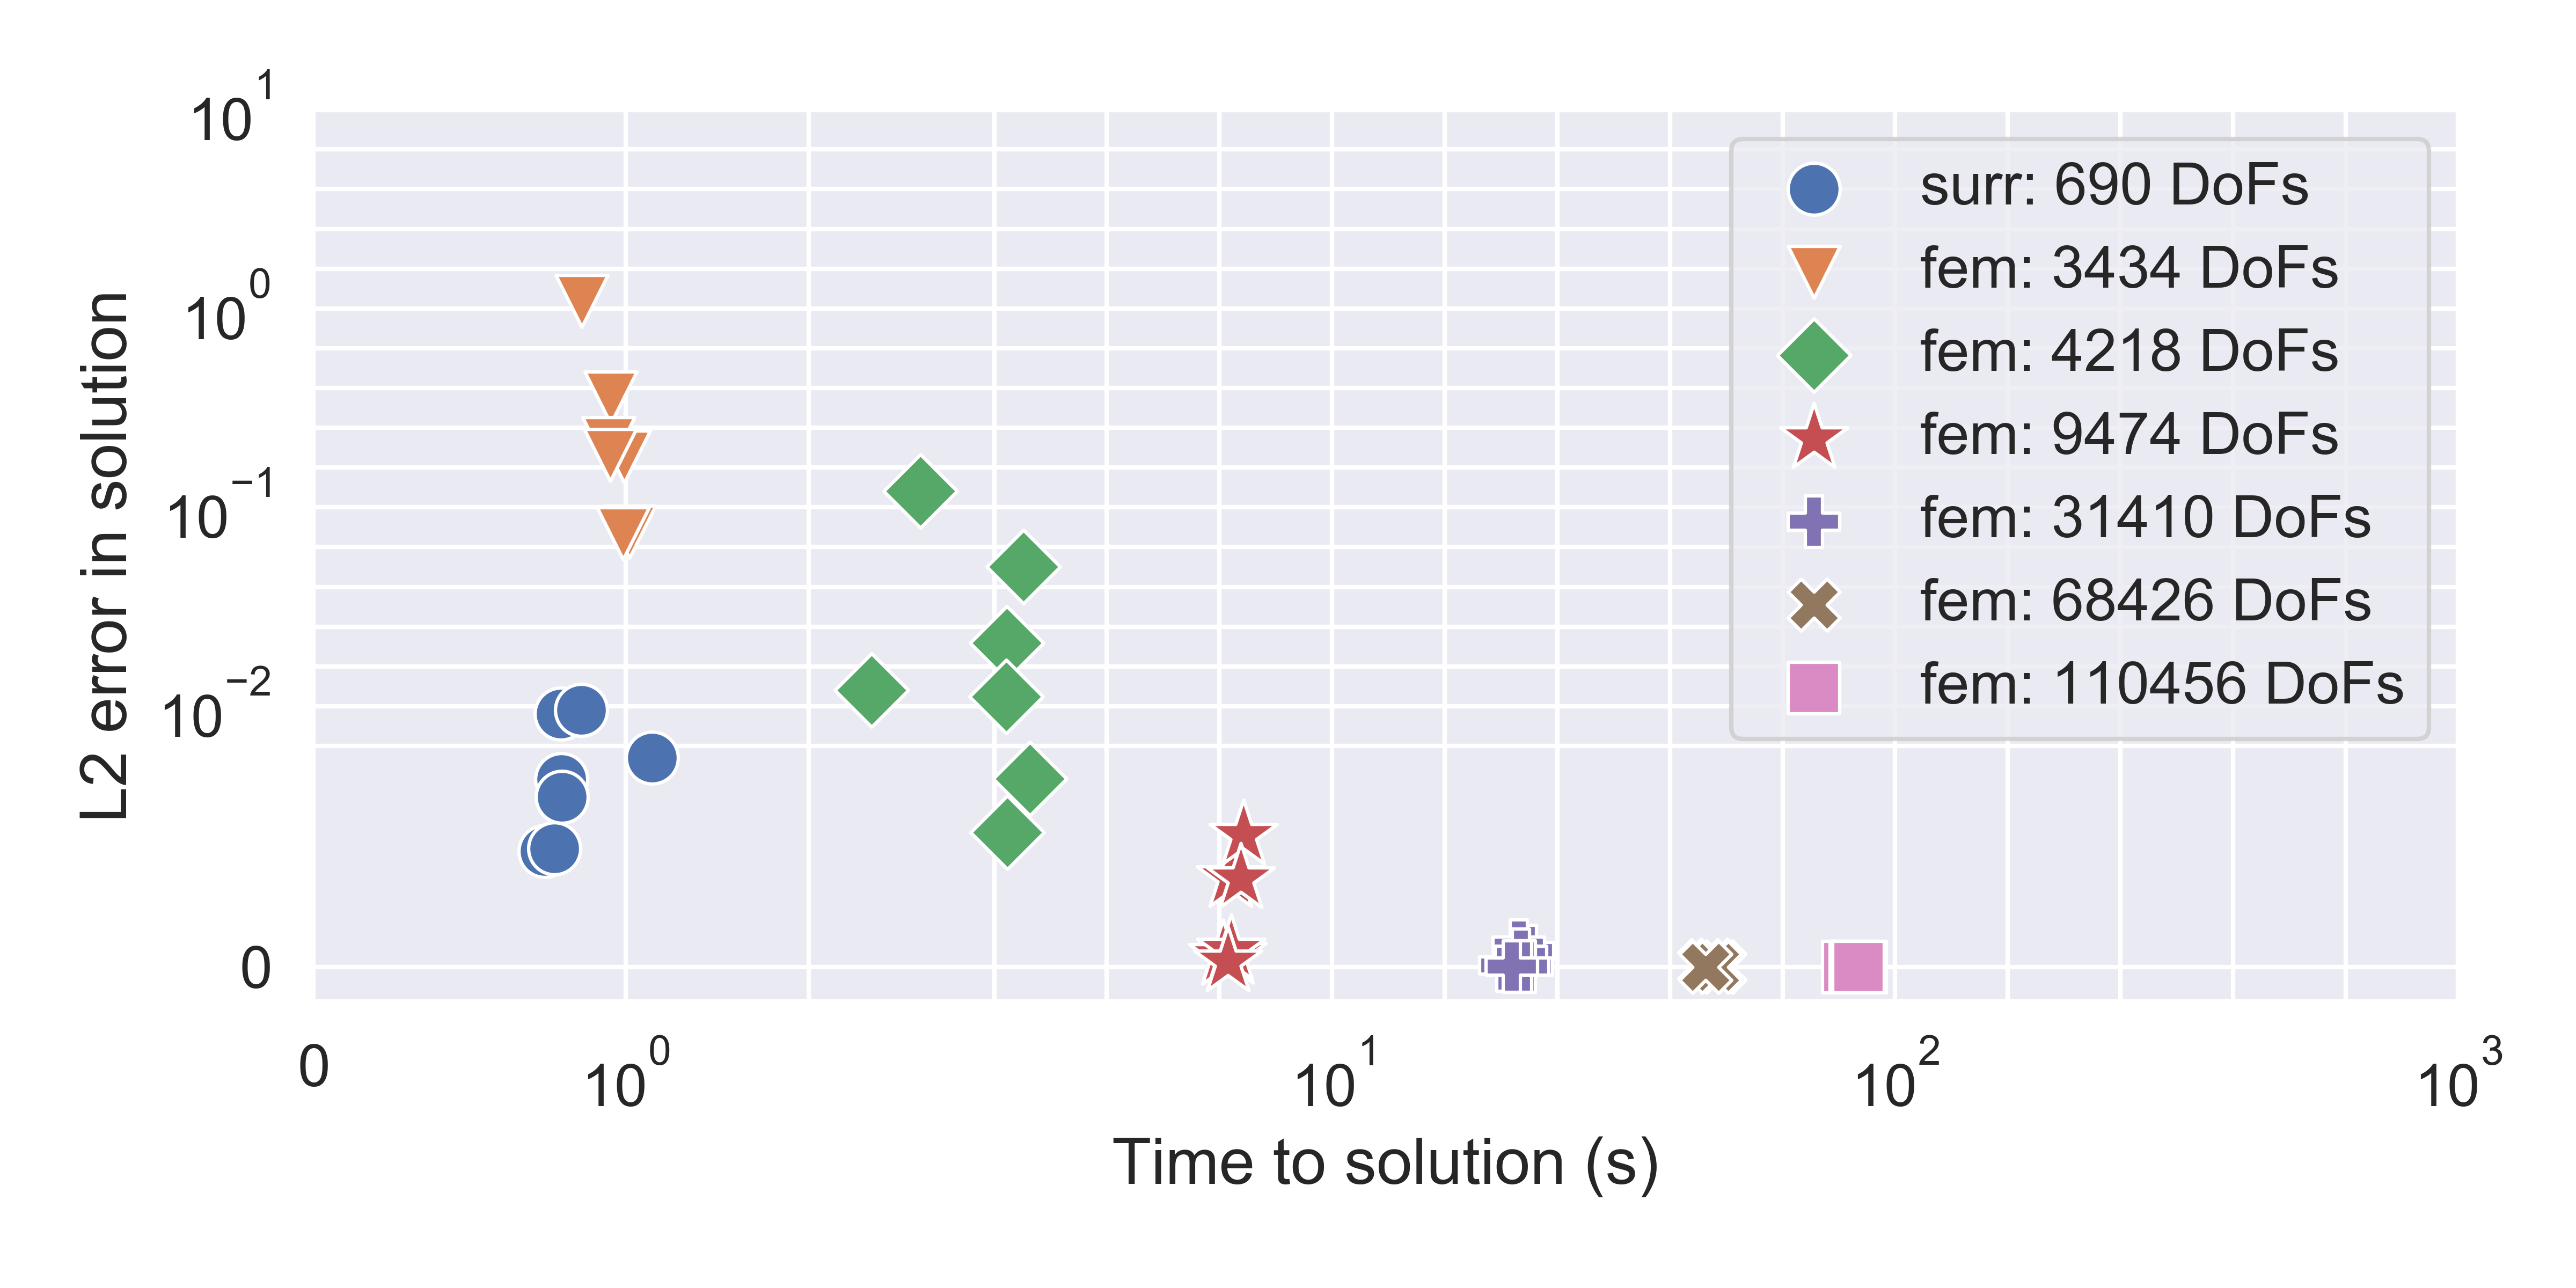
\includegraphics{lces/figures/tension_err.png}
	 \end{adjustbox}
	}}
\end{tabular}
	\vspace{-0.5cm}%
	\caption{\small Error in solution and in estimated energy vs solution wall clock time for the composed energy surrogate and for finite element models with varying mesh sizes. Top: axial compression. Bottom: axial tension.}%
	\label{fig:results}%
 \vspace{-0.3cm}
\end{figure*}

We use PyTorch's L-BFGS routine to minimize the composed surrogate energy, with step size $0.25$ and default criteria for checking convergence. We attempt to solve each finite element model with FEniCS' Newton method with $[1, 2, 5, 10, 20]$ load steps and relaxation parameters $[0.9, 0.7, 0.4, 0.1, 0.05]$, and record time taken for the \emph{fastest} convergent solve.
% We also tried the quasi-Newton method of PETSc \citep{petsc-web-page}, which often did not converge.
Under compression these solids exhibit nonlinear behavior, and only more conservative solves converge. Under tension they behave closer to a linear elastic model, and Newton's method converges quickly. Measurements are taken on an AWS M4.xlarge EC2 CPU instance. Using a GPU could provide further acceleration.
\begin{wrapfigure}[14]{r}{0.34\textwidth}
 \begin{tabular}{c|c}
	 {\resizebox{0.40\linewidth}{!}{
 \begin{adjustbox}{clip, trim=3.35cm 1.7cm 2.7cm 1.8cm}
	 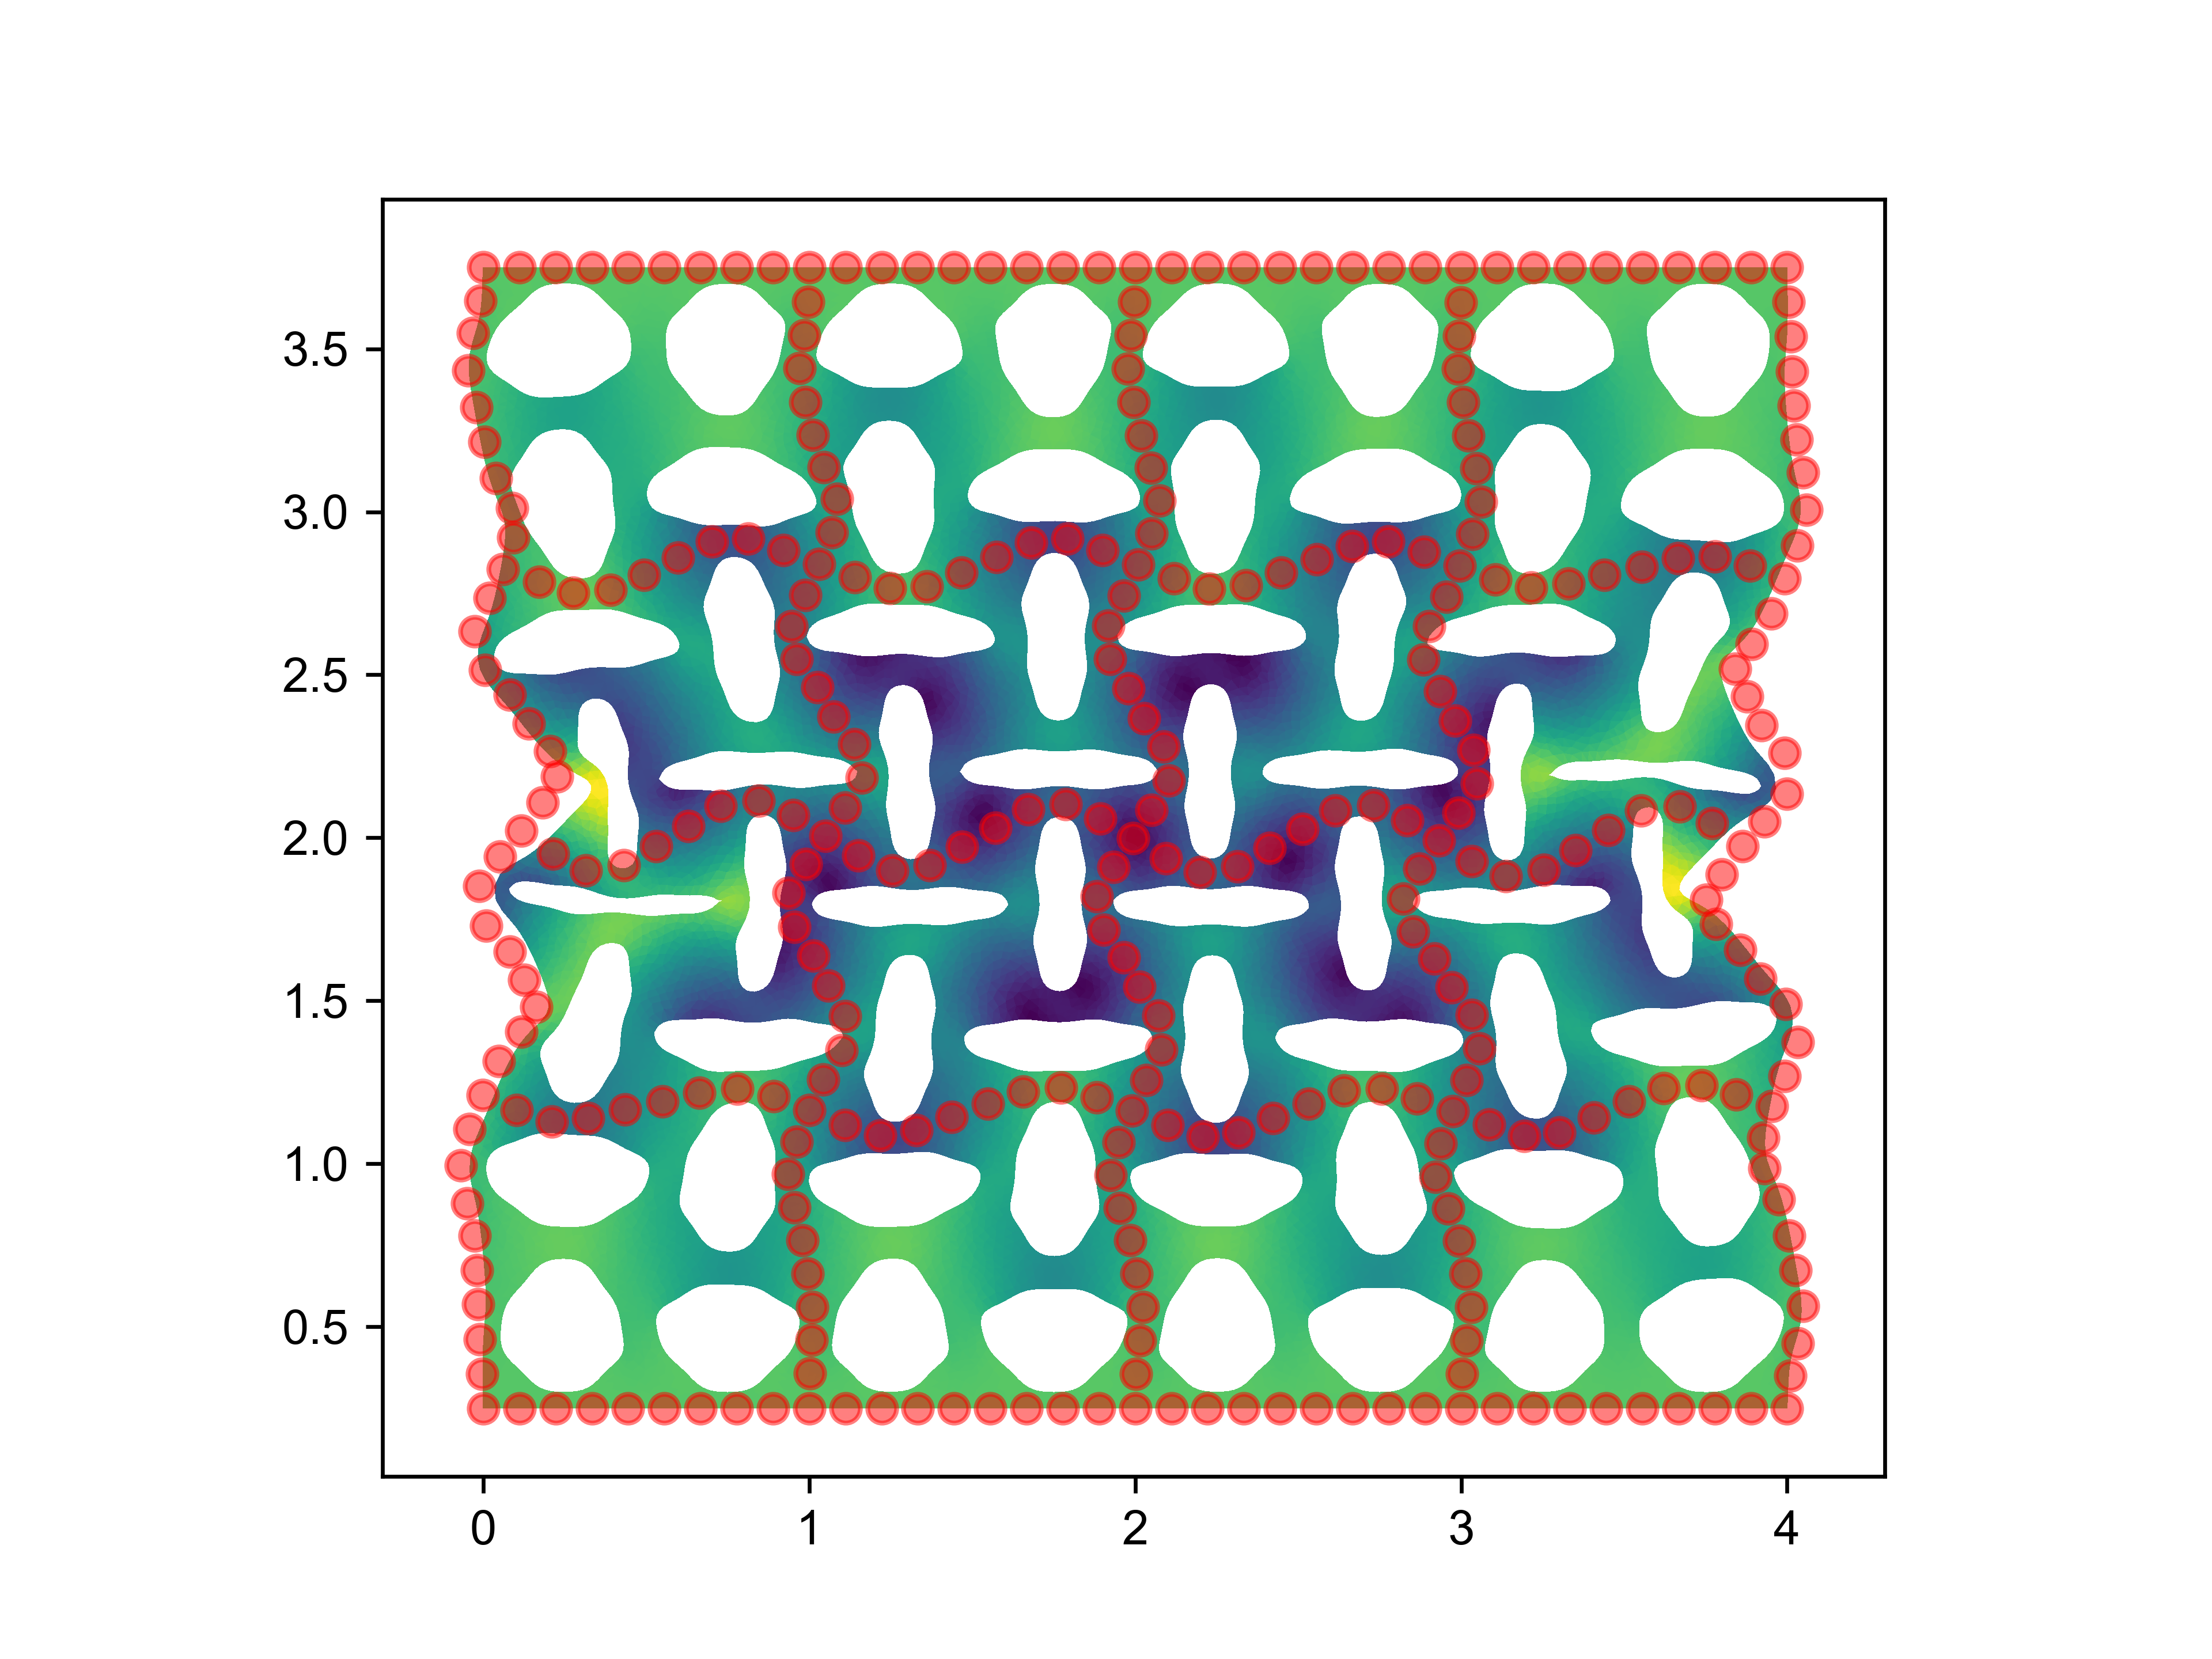
\includegraphics{lces/figures/compress_1.png}
	 \end{adjustbox}
	 }}&
	{\resizebox{0.45\linewidth}{!}{
 \begin{adjustbox}{clip, trim=2.2cm 1.7cm 2.3cm 1.8cm}
	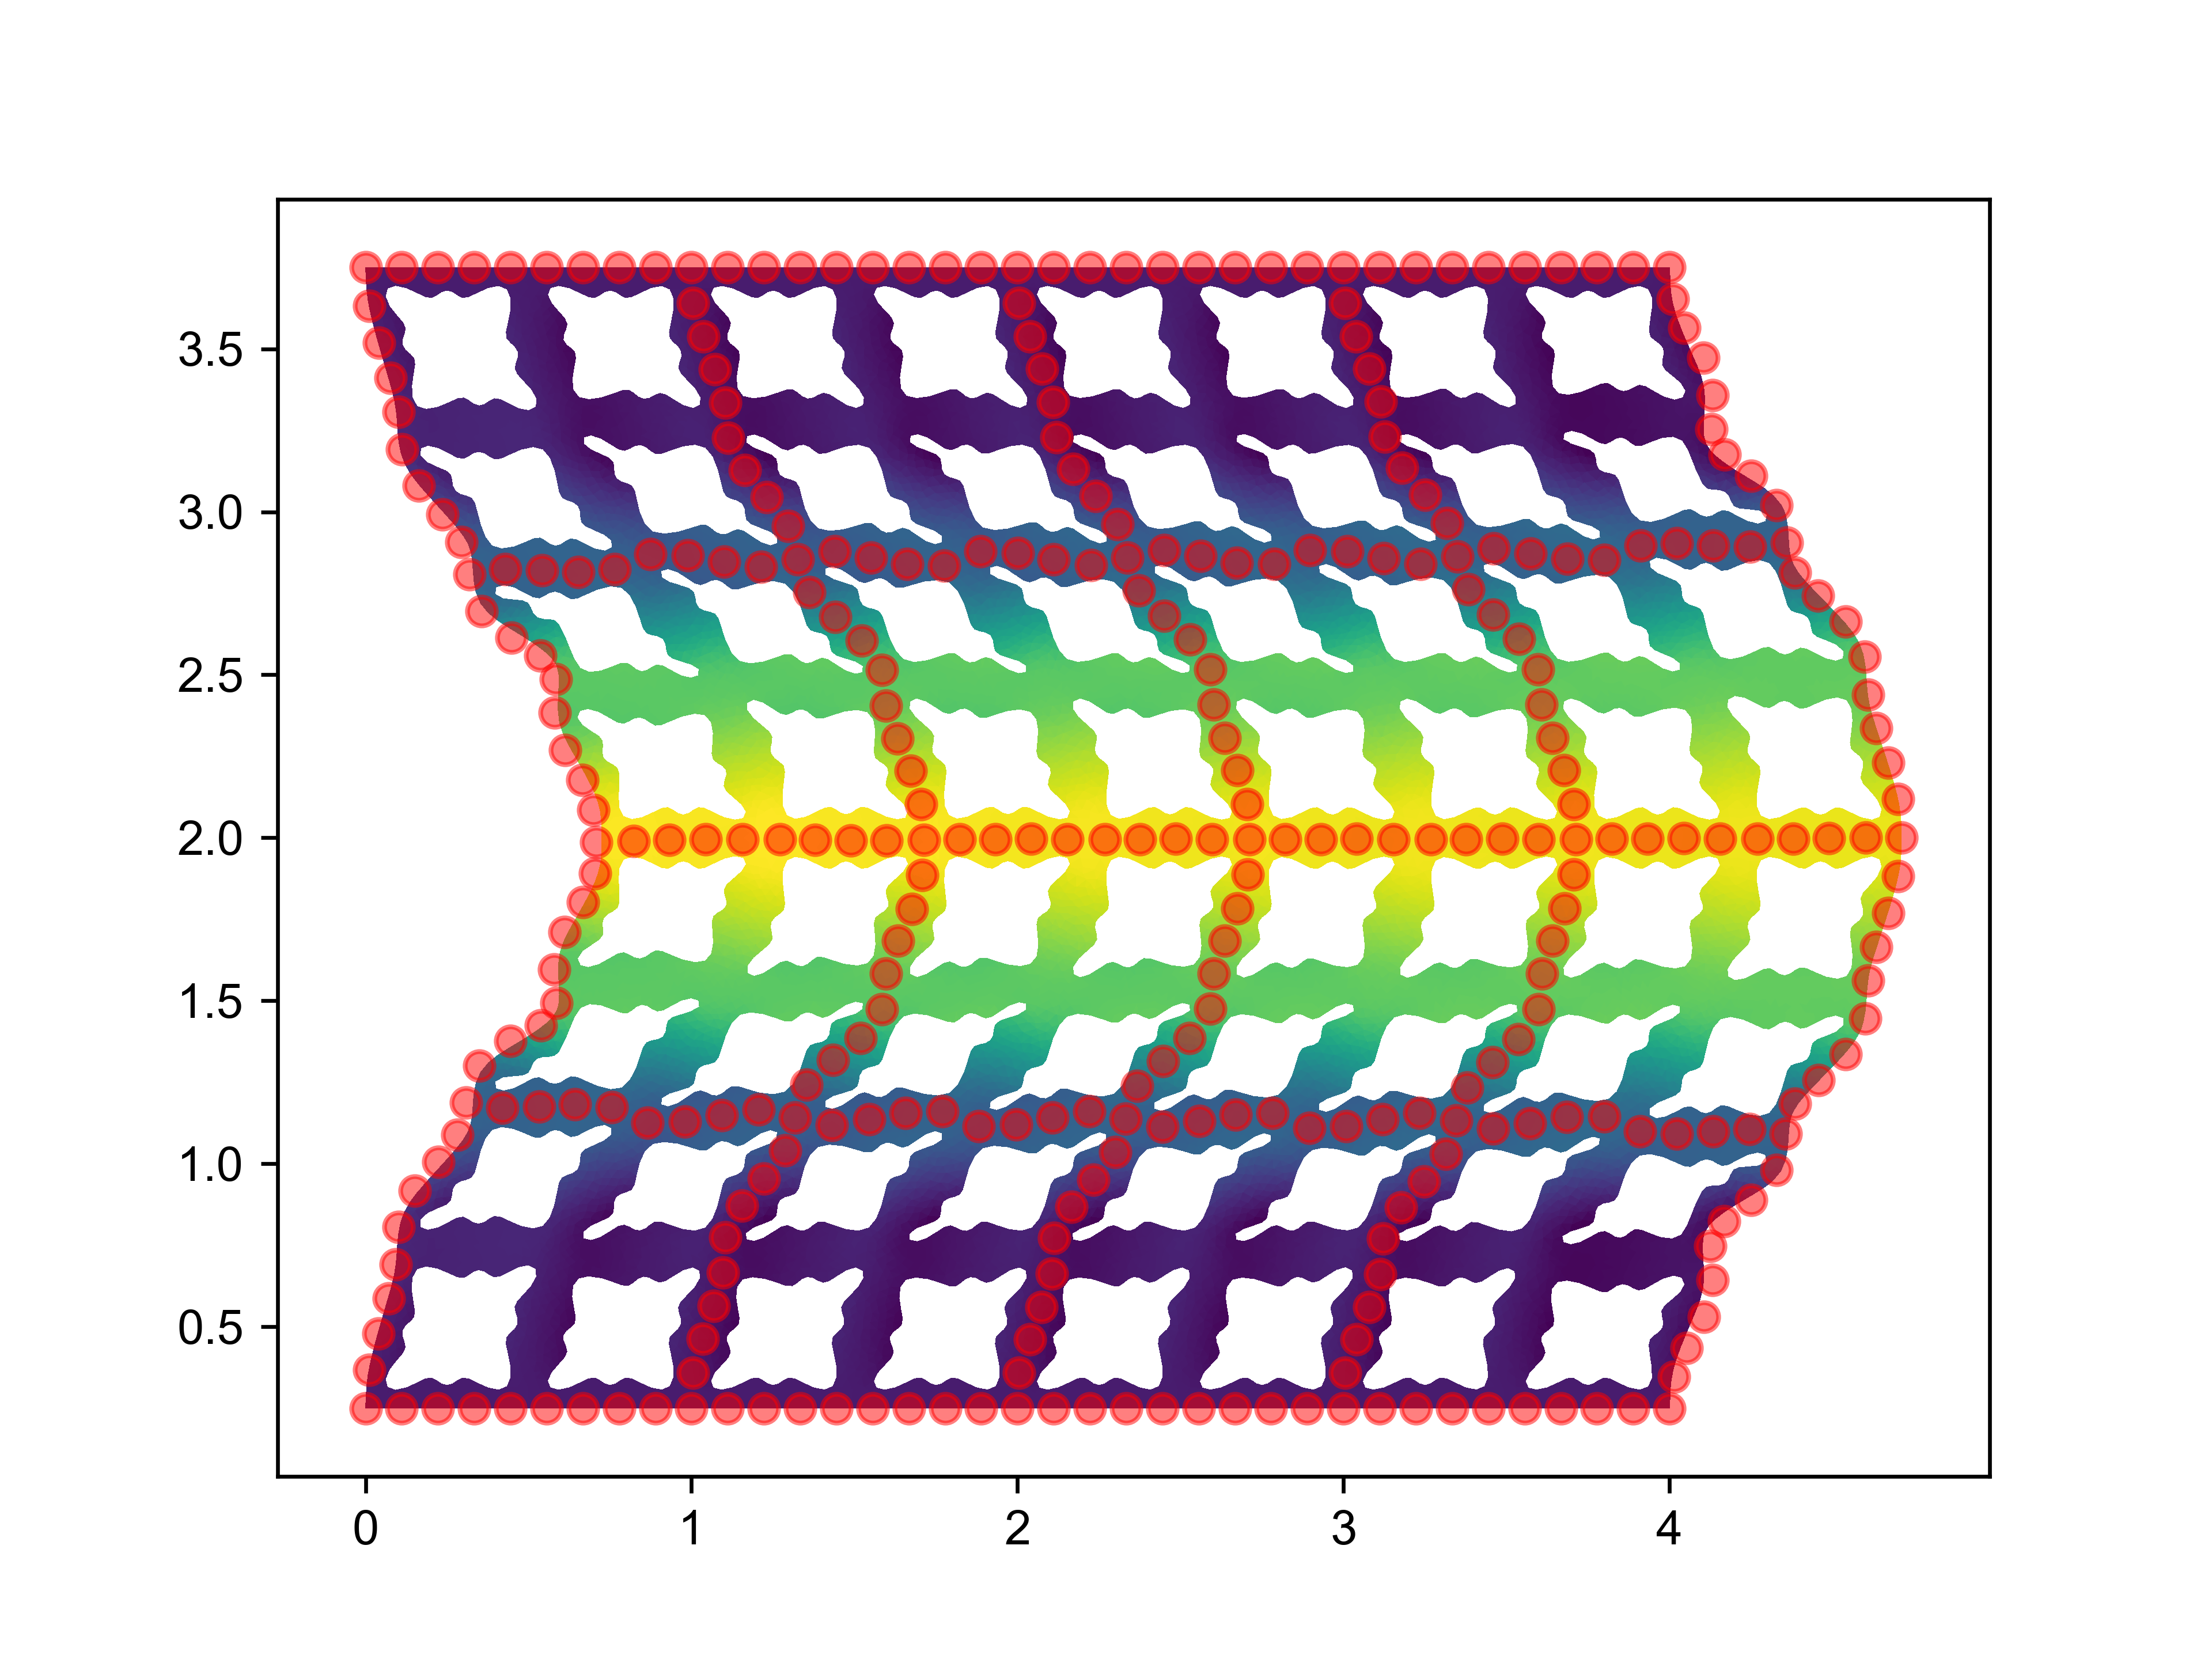
\includegraphics{lces/figures/compress_2.png}
	 \end{adjustbox}
	}}\\\hline
		\rule{0pt}{13ex}
	 {\resizebox{0.33\linewidth}{!}{
 \begin{adjustbox}{clip, trim=4.5cm 1.5cm 4.0cm 1.5cm}
	 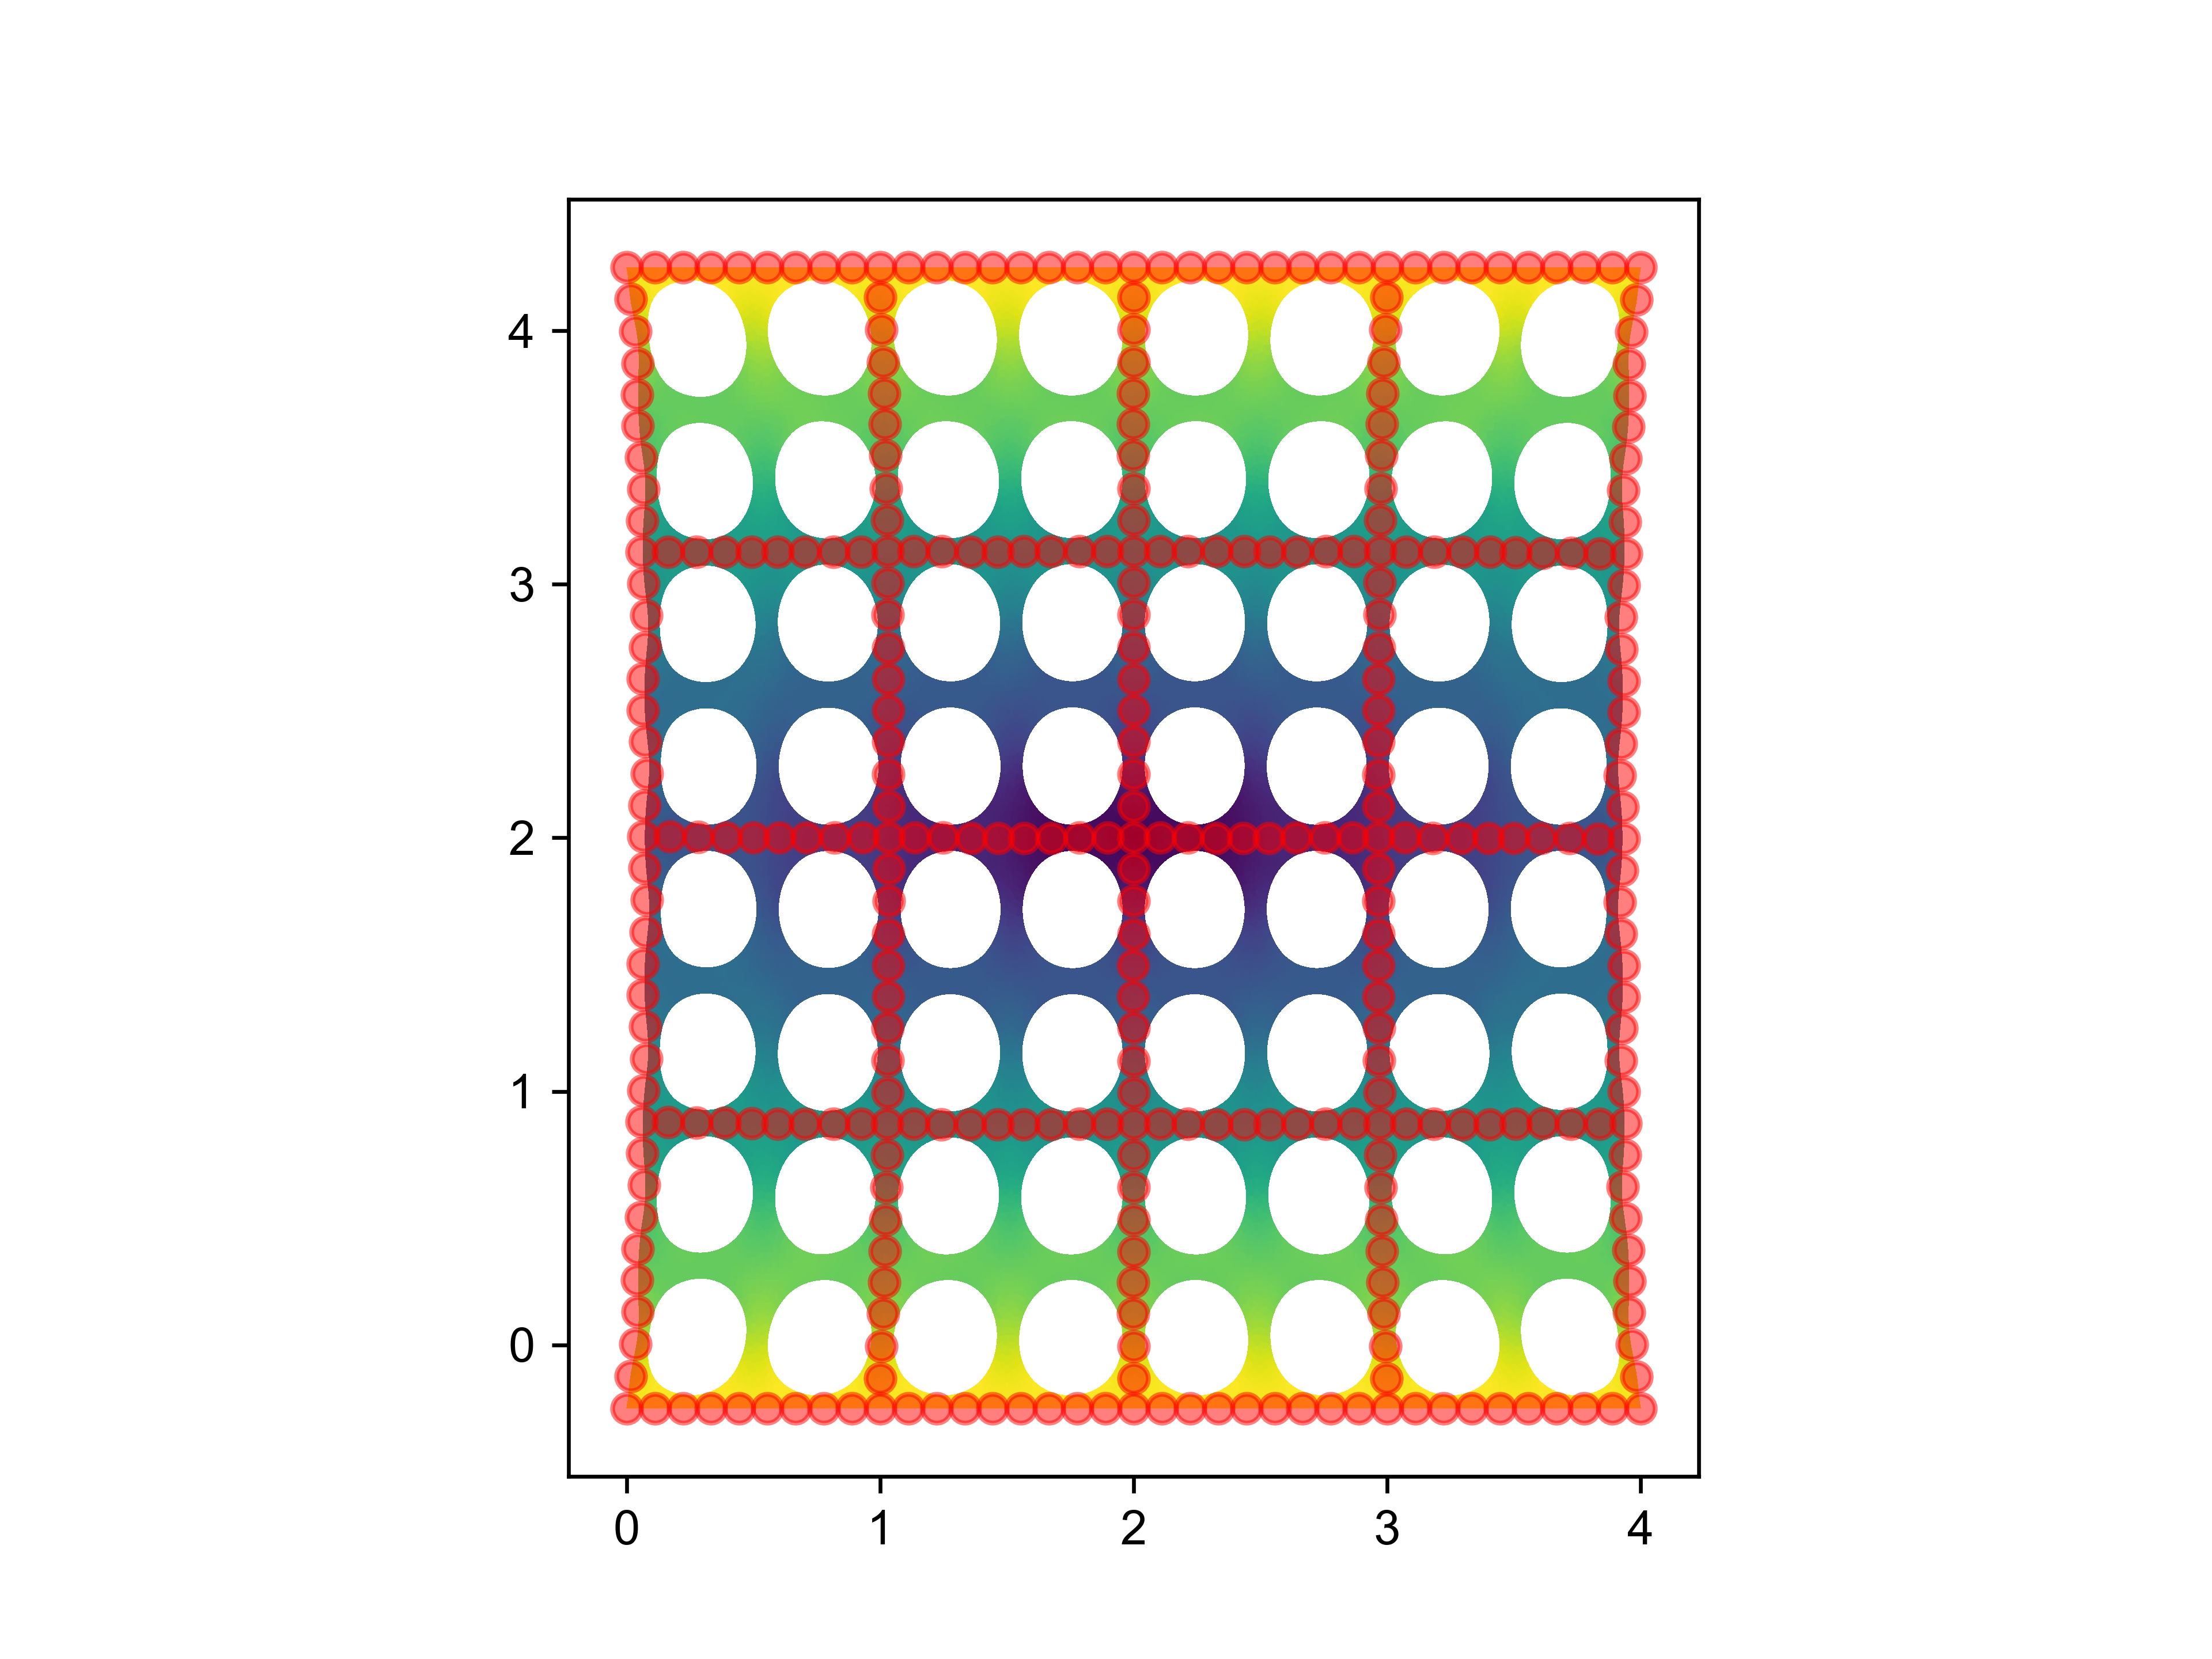
\includegraphics{lces/figures/tension_2.png}
	 \end{adjustbox}
	 }}&
	{\resizebox{0.33\linewidth}{!}{
 \begin{adjustbox}{clip, trim=4.5cm 1.5cm 4.0cm 1.5cm}
	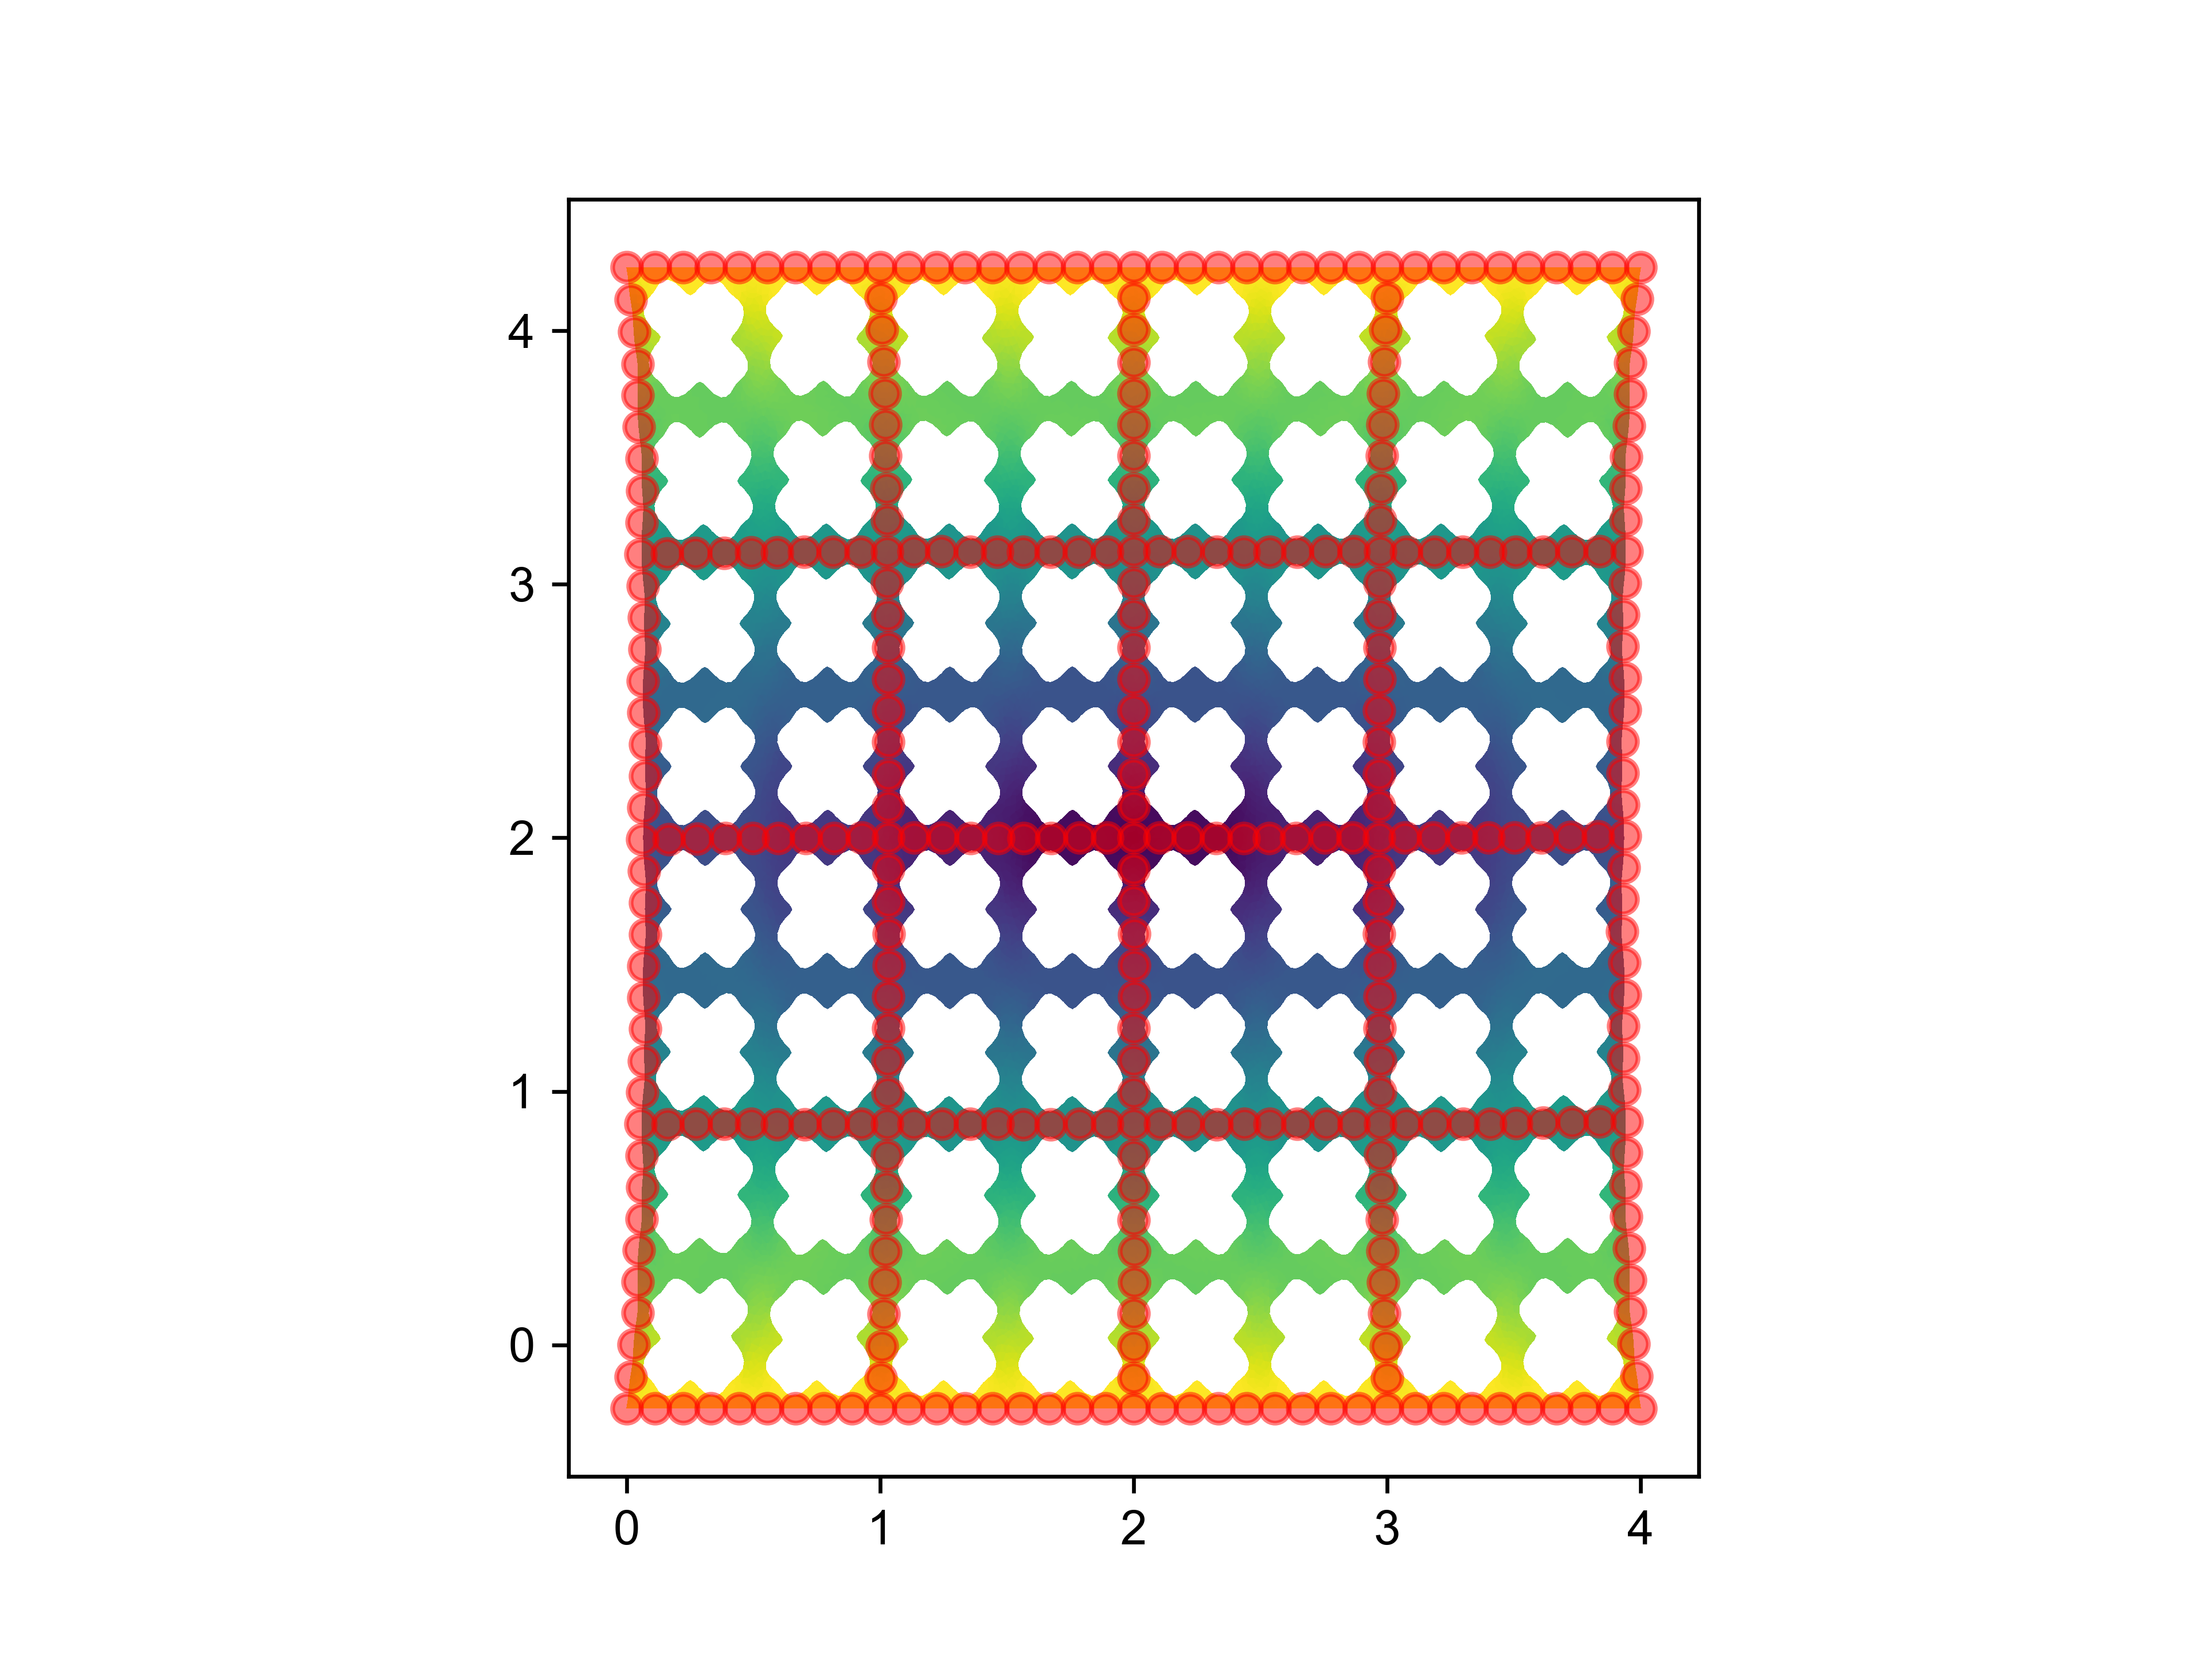
\includegraphics{lces/figures/tension_1.png}
	 \end{adjustbox}
	}}
\end{tabular}
\vspace{-0.3cm}
\caption{\small Meta-materials under compression (top) and tension (bottom), with solution found via CES shown in red at spline control points.}
\vspace{-0.8cm}
\label{fig:compress}
\end{wrapfigure}

We measure error in the solution and in the macroscopic energy. The former is~${||\hat{u}-u^*||_2^2}$, where $\hat{u}$ and $u^*$ are the approximation and ground-truth evaluated at spline control points. The latter is the relative error $\nicefrac{|\hat{E}(\hat{u}) - E^*(u^*)|}{E^*(u^*)}$, where $\hat{E}(\hat{u})$ is the approximated energy of the approximate solution, and $E^*(u^*)$ is the ground-truth energy of the ground-truth solution. As the energy function determines behavior, accuracy of energy is a potential indicator of ability to generalize to larger structures. The highest-fidelity finite element model is taken as ground truth, and thus has an error of zero on both metrics. Multiple minimizers exist as energy is preserved under rigid body transforms, so before comparing a solution~$\hat{u}$ to the ground-truth~$u^*$ we check each vertical and horizontal flip and use the flip which minimizes the solution error.
% \vspace{-0.2cm}

Figure \ref{fig:results} shows our evaluation. Composed energy surrogates are more efficient than high-fidelity FEA simulations yet more accurate than low-fidelity simulations. CES produces solutions with equivalent~$\ell^2$ error to FEA solutions which use an order of magnitude more variables or computation time, and with an order of magnitude less~$\ell^2$ error than FEM solutions requiring the same computation. This gap increases to several orders of magnitude when we consider percentage error in the predicted strain energy. We visualize the ground-truth and the CES approximation in Figure \ref{fig:compress}. See the appendix for visualization of FEM and CES solutions for the remaining structures.
